\documentclass[BSc]{usydthesis}

%%%%%%%%%%%%%%%%%%%%%%%%%%%%%%%%%%%%%%%%%%%%%%%%%%%%%%%%

\author{Ragib Zaman}
\title{Regression Models for Compositional Data}

%%%%%%%%%%%%%%%%%%%%%%%%%%%%%%%%%%%%%%%%%%%%%%%%%%%%%%%%

% causes equations to be numbered as section.equation
\numberwithin{equation}{chapter}

\theoremstyle{remark}

\newtheorem{Definition}[equation]{Definition}
\newtheorem{Theorem}[equation]{Theorem}
\newtheorem{Proposition}[equation]{Proposition}
\newtheorem{Lemma}[equation]{Lemma}
\newtheorem{Corollary}[equation]{Corollary}

\newtheorem{Remark}[equation]{Remark}
\newtheorem{Example}[equation]{Example}


\usepackage{amsmath,amsfonts,amsthm,bm}

%%%%%%%%%%%%%%%%%%%%%%%%%%%%%%%%%%%%%%%%%%%%%%%%%%%%%%%%

% personal macros

% common spaces
\newcommand{\N}{\mathbb{N}}
\newcommand{\R}{\mathbb{R}}
\newcommand{\Sb}{\mathbb{S}}
\newcommand{\Hb}{\mathbb{H}}
\newcommand{\U}{\mathbb{U}}

\newcommand{\Lag}{\mathcal{L}}
\newcommand{\M}{\mathbf{\mu}}
\newcommand{\E}{\mathbb{E}}
\newcommand{\x}{\mathbf{x}}

\DeclareMathOperator{\im}{im}
% for f:X -> Y; the default spacing isn't great
\newcommand{\map}[2]{\,{:}\,#1\!\longrightarrow\!#2}
\newcommand{\B}[1]{\mathbf{#1}}
% example \varphi \map{X}{Y}

%%%%%%%%%%%%%%%%%%%%%%%%%%%%%%%%%%%%%%%%%%%%%%%%%%%%%%%%

\begin{document}  

% roman page numbers for the initial pages
\pagenumbering{roman}

\maketitle          % creates the title page

\chapter*{Acknowledgements}
First and foremost I would like to thank Dr. Cheng Soon Ong. I greatly value the wisdom he has shared with me, helping me identify the core ideas of machine learning and the links in between. His willingness to give his time so generously and with such patience has been very much appreciated.\\

I would also like to thank Dr. Weifa Liang and Dr. Stephen Gould for taking the responsibilities of course convener and examiner respectively. Without their contribution I would not have been able to have the pleasure of completing this course. 

\chapter*{Abstract}
In this report we explore regression models involving compositional data. We provide some background of the standard methods of analysing compositional data originally developed primarily by Aitchison (1982, 1986) and Egozcue (2003). After surveying regression problems involving compositions and models for studying them, we give particular focus to a problem we call Aitchison Simplex Regression, where all variables are compositions within the same simplex. A model for this problem was introduced by Wang et al. (2013). In this report we propose several new models for this problem, incorporating bias terms and gauged-KL divergence loss functions.\\ 



\tableofcontents    % creates the table of contents

% reset the page numbering and change to arabic numbers
\newpage\setcounter{page}{1}\pagenumbering{arabic}

\chapter{Introduction}
Compositions are data which contain the information of the relative proportions of multiple parts which together form a whole. They commonly arise in fields such as chemistry, biology, geology and election forecasting, where samples are taken from an object due to it being impractical or unnecessary to take measurement of the entire object. In compositions the relative proportions of the parts contain the meaningful information rather than the actual values of the parts themselves. Thus, compositions are invariant under scaling of all the components by some positive factor.\\

In machine learning we attempt to analyse data to perform tasks such as regression or dimensionality reduction, however standard methods such as linear regression and principal component analysis (PCA) often require that the data naturally resides in some Euclidean space $\mathbb{R}^d,$ which compositions do not. The most naive approach to modelling compositions is to simply forget their special structure and use whichever raw numbers are provided in the original data. This is problematic, since the models in standard methods are not invariant under positive scaling of the input data, so we may get different results depending on how the original data was chosen to be represented. Although there are obvious approaches to get around this (such as normalising the data so the components always sum to $1$), there are still several issues.\\

 \begin{itemize}
  \item The model functions of standard methods often require us to add points together and multiply by real coefficients. The usual vector space operations of $\mathbb{R}^d$ do not apply naturally to compositions. For example, scalar multiplication reduces to the identity map. We require a natural vector space structure on the probablity simplex to use similar model functions to the standard ones.\\
 \item To minimise the standard loss functions we require a suitable notion of distance for compositions. While we could forget the special structure of compositions and, for example, use the Euclidean metric on normalised points, it is unclear whether this is appropriate.\\
  \item Compositions lie in a strict subspace of Euclidean space, as their components always sum to some fixed constant. This means that the data matrices do not have full rank and have a singular covariance matrix, which can bring issues related to uniqueness and/or numerical stability in certain machine learning algorithms.\\ 
 \end{itemize}
 
Even if one could directly apply a standard method, it is natural to expect that a model which specifically addresses and/or incorporates the special structure of compositions will outperform a model which ignores it. In the first systematic treatments of the statistics of compositional data, Aitchison (1982, 1986) defined a Hilbert space structure on compositions and introduced the centred log-ratio transform which naturally maps compositions to a subspace of Euclidean space subject to a constraint. Egozcue et al. (2003) extended this by introducing the isometric log-ratio transform which removed the constraint and gave a natural way to derive Aitchison's Hilbert space structure. Although this allows us to transform compositions into Euclidean data, it may not always be most appropriate to measure the distance between compositions by the Euclidean distance between the transformed points. Avalos-Fernandez et al. (2018) studied PCA on compositional data, measuring quality of fit of a subspace by a general Bregman divergence and giving evidence that using the Kullback-Liebler divergence may be a desirable alternative in some applications.\\

After setting up some required background, we investigate regression problems involving compositional data. Of particular interest is modelling a dependent compositional variable as a function of multiple independent compositional variables. We review a model introduced by Wang et al. (2013) before introducing some new models for this problem. 
 
 
 
\chapter{Background}

In this chapter we define compositions and the essential spaces and operations that are commonly used to manipulate them. These will give us a better understanding of what regression models involving compositions may look like and will be used heavily in the next chapter.

\section{Definition and Examples}
\begin{Definition}
Let $d$ be a positive integer. Let $\sim$ be the equivalence relation on the positive orthant $\mathbb{R}^d_{\geq 0}$ where for $x, x' \in \mathbb{R}^d_{\geq 0}$ we have $x \sim x'$ if and only if $x = \lambda x'$ for some $\lambda > 0.$ A $d$-part composition is an element of the quotient set $\mathbb{R}^d_{\geq 0}/\sim.$ 
\end{Definition}

We refer the reader to Herstein (1975) for a concise discussion on equivalence relations, equivalence classes and quotient sets, although they have get the essential idea from the examples below.

\begin{Example}
In a two party election we may survey members of various electorates for their preferred party and collect the following results.

\begin{table}[hbt!]
\centering
\begin{tabular}{|l|l|l|} 
\hline
Electorate   & Party A & Party B  \\ 
\hline
Electorate 1 &   23    &   31     \\
Electorate 2 &   34    &   27     \\
Electorate 3 &   13    &   15     \\
\hline
\end{tabular}
\end{table}

The data points for each electorate may be regarded as a 2-part composition. For Electorate 1 the point is $[(23,31)].$ If the total votes in Electorate 1 for Party A and Party B were instead 46 and 62 respectively, our data point would be the same composition since $[(23,31)] = [(46,62)].$ 
\end{Example}

\begin{Example}

Four common varieties of steel have approximate elemental compositions as below. If we took a 10 gram sample of a piece of steel whose variety is not known and it contained 0.015 grams of Carbon, 0.035 grams of Manganese and 9.95 grams of Iron, we may classify it as Mild Carbon, as $[(0.015, 0.035, 9.95)] = [(0.15, 0.35, 99.5)].$

\begin{table}[hbt!]
\centering
\begin{tabular}{|l|l|l|l|} 
\hline
Steel Variant    & \% Carbon & \% Manganese & \% Iron  \\ 
\hline
Mild Carbon      & 0.15      & 0.35         & 99.50    \\
Medium Carbon    & 0.4       & 0.9          & 98.7     \\
High Carbon      & 0.7       & 0.8          & 98.5     \\
Very High Carbon & 1.5       & 1.0          & 97.5     \\
\hline
\end{tabular}
\end{table}
\end{Example}

\begin{Example}
Three super funds have invested their assets into economic sectors as below (amounts are MM \$AUD). Fund A and Fund C have the same composition and we may expect their Return on Investment (ROI) to be similar. 
 \begin{table}[hbt!]
\centering
\begin{tabular}{|l|l|l|l|} 
\hline
Super Fund & Technology & Real Estate & Other Sectors   \\ 
\hline
Fund A     & 233.3      & 45.2        & 432.3           \\
Fund B     & 154.3      & 64.6        & 356.7           \\
Fund C     & 699.9      & 135.6       & 1296.9          \\
\hline
\end{tabular}
\end{table}
\end{Example}
\begin{Remark}
When we understand that a point is a composition we usually omit the brackets. 
\end{Remark}

\section{Coordinates and transformations for compositions}

We now present a set of coordinate systems and maps between them which help in the analysis of compositions. Many operations on compositions try to map compositions bijectively over to spaces that are closer to Euclidean space, so that we can apply known techniques and avoid complications of quotient spaces. These operations usually require that all the components of a composition are non-zero, and would lead to infinite values otherwise. Thus, most treatments of compositional data proceed with this assumption of strictly positive components in their analysis. In practice most measurements have some amount of error associated to them and the target they try to analyse varies continuously with respect to the components, which they use to justify replacing any zero components with a small positive value. This value is often chosen somewhat arbitrarily (such as by Avalos-Fernandez et al. (2016) and Wang et al. (2013)). Martin-Fernandez (2003) studied a systemic approach to choosing this value and gave some arguments towards its suitability, and this method is now offered in statistical computing packages (such as Scikit-Bio's 'Compositions' package for Python (Scikit-Bio 2019), and the 'compositions' package for R (CRAN 2019)) as the primary way to dealing with zero values. Some studies involving compositional data use techniques which can deal with zero components directly such as that by Scealy \& Welsh (2014). For the rest of this report we assume our compositions have no zero valued components. 

\begin{Definition}
 We define the following spaces.
 \begin{align*}
  S^d &= \bigg\{ x \in \mathbb{R}_{>0}^d \ \bigg| \ \sum_{i=1}^d x_i = 1 \bigg\} \\
  H^d &= \bigg\{ x \in \mathbb{R}_{>0}^d \ \bigg| \ \prod_{i=1}^d x_i = 1 \bigg\} \\
  U^d &= \bigg\{ x \in \mathbb{R}^d \ \ \ \bigg| \ \sum_{i=1}^d x_i = 0 \bigg\} \\
 \end{align*}
The space $S^d$ is the interior of the probability simplex, and in the context of compositional data analysis is sometimes called the 'Aitchison space/complex/geometry' although we reserve this term for when this space is endowed with the Hilbert space structure described in the next section. The space $H^d$ is generally not named, though we may say a composition in this space is given in hyperbolic coordinates. The hyperplane $U^d$ is sometimes called the clr-plane. 
\end{Definition}

The oblique hyperplane $U^d$ has dimension $d-1,$ and by applying a rotation we can isometrically map $U^d$ to the $d-1$ dimensional subspace of $\mathbb{R}^{d}$ defined by $x_d=0.$ We fix one particular rotation, a $(d-1) \times d$ matrix $W$ such that $WW^T = I_{d-1}$ and $W^TW = I_d - \frac{1}{d} \mathbf{1}_{d\times d},$ which is obtained through a Gram-Scmidt process described by Egozcue (2003). Any other rotation $W'$ with these properties could be used in place of $W$ however $W$ is simple to compute and using other $W'$ can be seen as applying $W$ and then further flipping, rotating or shifting the space $\mathbb{R}^{d-1},$ which provides no additional benefit for data analysis (Egozcue 2003). 


\begin{Definition}
 Define $g(x)$ to be the geometric mean of the components of $x,$ and interpret $\exp$ and $\log$ functions on a vector as component-wise application. We define a sequence of maps between the coodinate spaces.   \\

$ \scalebox{1.5}{$ \R^d_{> 0}/\sim \ \  \xrightarrow[{[x]\mapsto \frac{1}{\| x\|_1} x }]{{\mathcal{C}}} S^d \  \xrightarrow[{x \mapsto \frac{x}{g(x)}}]{{\tilde{\cdot}}} \ H^d \xrightarrow[{x \mapsto \log x}]{{\log}}\ U^d \ \xrightarrow[{x\mapsto Wx}]{{W}}\ \R^{d-1} $}$
\\
\\
\\
\\
$ \scalebox{1.5}{$ \ \ \ \  \R^d_{> 0}/\sim \ \ \ \ \xleftarrow[{x\mapsto [x] }]{\text{quotient}} \ \ \  S^d \xleftarrow[{x \mapsto \frac{1}{\| x\|_1} x}]{{\mathcal{C}'}} H^d \xleftarrow[{x \mapsto \exp x}]{{\exp}} U^d \xleftarrow[{x\mapsto W^Tx}]{{W^T}}\R^{d-1} $}$
\end{Definition}

All maps in the above definition are well-defined, continuous and bijective (with their inverse function given by the map in the opposite direction). Through these maps, we can transform a composition into coordinates expressed in any of the above spaces. The centred log-ratio map 
\begin{align*}
 clr : S^d &\to U^d \\
    x &\mapsto \log \frac{x}{g(x)}
\end{align*} 
was introduced by Aitchison (1982) and the isometric log-ratio map 
\begin{align*}
 ilr : S^d &\to \mathbb{R}^{d-1} \\
    x &\mapsto W \log \frac{x}{g(x)}
\end{align*}
was introduced by Egozcue (2003). Both of these maps (and their inverses) can be seen as compositions of consecutive maps in the definition above. Since these maps have been introduced, the standard approach to analysing compositional data has been to apply classical machine learning techniques to the transformed coordinates. Some of those techniques can be given an interpretation strictly within the Aitchison simplex $S^d.$


\section{Hilbert Space Structure of the Aitchison Simplex}
Recall that if $X$ and $Y$ are two topological spaces, a map $f:X\to Y$ is called a homeomorphism if it is a continuous bijective map whose inverse is also continuous. The existence of a homeomorphism between $X$ and $Y$ indicates that $X$ and $Y$ are equivalent in terms of topological structure. The isometric log-ratio function provides a homeomorphism from $S^d$ to $\mathbb{R}^{d-1},$ and through this map we can also transport the Hilbert space structure of $\mathbb{R}^{d-1}$ onto $S^d.$ 

\begin{Proposition}
 Let $X$ be a topological space and $H$ be a Hilbert space with addition, scalar multiplication and the inner product of $H$ denoted by $+,\  \cdot$ and $ \langle \cdot, \cdot \rangle$ respectively. Let $f: X \to H$ be a homeomorphism. Define the maps
\begin{align*}
 \odot : \mathbb{R} \times X &\to X \\
    \alpha \odot x &= f^{-1}( \alpha \cdot f(x) )\\
    \ \\
 \oplus : X \times X &\to X \\
    x \oplus x' &= f^{-1}( f(x) + f(x'))\\
    \ \\
 \langle \cdot, \cdot \rangle_X : X \times X &\to \mathbb{R}_{\geq 0} \\
    \langle x, x' \rangle_X &= \langle f(x), f(x') \rangle
\end{align*}
Then, equipped with those maps, $X$ is a Hilbert space and $f$ is an isometry between $X$ and $H.$
\end{Proposition}

\begin{proof}
 It is trivial to verify that the defined maps satisfy the axioms of an inner product space. Now we check that $X$ is a Hilbert space, that is we verify that $X$ is a complete metric space under the metric induced by the inner product. Let $(x_n)$ be a Cauchy sequence in $X,$ and fix an arbitrary value $\epsilon > 0.$ By the continuity of $f,$ there exists a $\delta>0$ such that $\| f(x) - f(x') \| < \epsilon$ for all $x, x' \in X$ such that $\| x\ominus x'\|_X < \delta.$ Since $(x_n)$ is a Cauchy sequence, there exists a positive integer $N$ such that $\| x_n \ominus x_m \|_X < \delta$ for all $n,m > N.$ Hence we have $\| f(x_n) - f(x_m) \| < \epsilon$ for all $n,m > N,$ proving that $f(x_n)$ is a Cauchy sequence in $H.$ Therefore, $f(x_n) \to z$ for some $z\in H.$ By the definition of the inner product of $X,$ we have $\| f^{-1}(z) \ominus x_n \|_X = \| z - f(x_n) \| \to 0$ so $(x_n)$ converges in $X,$ proving the claim that $X$ is a Hilbert space. The fact that $f$ is an isometry between $X$ and $H$ is essentially a tautology given how we have defined the inner product of $X.$
\end{proof}

Applying this to the isometric log-ratio transform, equipping the following operations onto the Aitchison simplex $S^d$ produces a Hilbert space.  
\begin{align*}
 \odot : \mathbb{R} \times S^d &\to S^d \\
    \alpha \odot x &= \frac{1}{\sum_{i} x_i^{\alpha}} [x_i^{\alpha}] \\
    \ \\
 \oplus : S^d \times S^d &\to S^d \\
    x \oplus x' &= \frac{1}{\sum_i x_i y_i} [x_i y_i] \\
    \ \\
 \langle \cdot, \cdot \rangle_a : S^d \times S^d &\to \mathbb{R}_{\geq 0} \\
    \langle x, x' \rangle_a &= \sum_{i=1}^d \log \left( \frac{x_i}{g(x)} \right)\log \left( \frac{y_i}{g(y)} \right)
\end{align*}

\begin{Example}
Suppose for example that $s, s' \in S^d$ with ilr coordinates $x, x' \in \mathbb{R}^{d-1}.$ A learning model may make predictions by linear combinations of the Euclidean vectors, say something of the form $\beta \cdot x + \beta' \cdot x',$ and then inverting the ilr transform. With the Hilbert space structure of the Aitchison simplex, this can instead be interpreted entirely as operations within the simplex - $\beta \odot s \oplus \beta' \odot.$ 
\end{Example}

\section{Centralisation}

In $\mathbb{R}^{d-1}$ we can define the centre of points $x_1,\ldots, x_n \in \mathbb{R}^{d-1}$ to be the mean $\frac{1}{n} \sum_{i=1}^n x_i.$ We can transfer this to define a centre of compositions.

\begin{Definition}
 Suppose $u_1, \ldots, u_n \in S^d$ are compositions. The centre of these points is given by 
 
$$ \overline{u} = \frac{1}{n} \odot \bigoplus_{i=1}^n u_i$$
To centralise a set of compositions, we subtract the centre from each element of the set. 
\end{Definition}

The following method is easily verified to be equivalent to but more computationally efficient than computing the centre from the above definition. First form the vector in $\mathbb{R}^d$ where the $i$-th component is the geometric mean of the $i$-th components of all the compositions in the set. Then normalise this vector so that it lies in $S^d.$ We can centre a set of compositions by subtracting their centre from each of them, and un-centre by adding the centre back. \\
\
We now have sufficient background to discuss regression problems involving compositional data and the various methods of approaching them.


\chapter{Regression with Compositions}

We now briefly define the possible forms of a regression problem involving compositions before we discuss the particular problem that was our focus. \\
\section{General regression}
In general, we may wish to estimate a continuous target (either a real number or a composition) given a set of real numbers and a set of compositions. More precisely, we may have 

\begin{itemize}
 \item A continuous target $y$ with either $y\in \mathbb{R}$ or $y\in S^{d_0}.$
 \item Independent compositional variables $s_1,\ldots, s_m$ where $s_i$ has $d_i$ parts.
 \item Independent real variables $x_1, \ldots, x_{m'}$.
\end{itemize}
 
A regression problem is to learn a function $f$ such that $f(s_1,\ldots, s_m, x_1, \ldots, x_{m'})$ gives a good estimate of the target variable $y,$ where the quality of an estimate is given by a predetermined loss function. Unfortunately there is no accepted convention for naming the various special cases of this regression problem.

\begin{Example}
 A common case is the problem of predicting a real value given a single independent compositional variable. For example, Aitchison (1986) studies the problem of using the relative sand/silt/clay composition of a sediment sample taken from an Arctic lake to estimate the depth in the lake from which the sample was taken. 
\end{Example}

\begin{Example}
 Another common case is the problem of predicting a composition given $m$ independent real variables. An example would be modelling the adult/child composition of a household, given their annual expenditure on 10 categories of retail goods. One model commonly used for this problem is the following:
 
 $$ b_0 \oplus \left( \bigoplus_{k=1}^m x_k \odot b_k \right)$$
 
 Here the learned parameters $b_i$ are compositions within the same simplex as the target, and the loss between the estimate and label is given by the distance within the Aitchison simplex. This model was first introduced by Aitchision \& Shen (1980) and the algorithm for computing the parameters has been greatly improved by Aitchision \& Egozcue (2005).
\end{Example}




\section{Aitchison Simplex Regression}

The case which is the main focus on this report is when we wish to model a target $y \in S^d$ given $m$ independent compositional variables $x_1,\ldots, x_m \in S^d.$ In this case, all of the inputs and outputs of the model lie within the same Aitchison simplex $S^d,$ and we call this problem Aitchison Simplex Regression. \\

A naive attempt at this problem would be to simply treat the the compositions as values in $\mathbb{R}^d$ and apply standard linear regression models. One quickly sees that if we do this, we produce outputs which are almost never compositions. Even intending to normalise the outputs is insufficient, as we can not normalise the output is even a single component is negative (which is often the case). The most promising approach forward is to think in terms of clr and ilr coordinates introduced in the previous chapter, and the following models make heavy use of these transformations.

\subsection{Model by Wang et al. (2013)}
Wang et al. (2013) proposed the following model for this problem:
$$ f(x_1, \ldots, x_m) = \bigoplus_{i=1}^m \beta_i \odot x_i $$ and provide a closed form solution for the parameters $\beta_i$ which minimise the error when the loss between an estimate and the true label is given by the Aitchison distance. Their derivation relies on the property that, when transformed by the ilr function, this model has a very particular form which reduces to the form of linear regression in Euclidean space. Note that this form does not accommodate learning a bias term. As a compromise, their method is to first pre-process all of the data by centralising all of the variables, training their model on this centred data, and then un-centre to form a prediction. 

\subsection{Bias learning model for Aitchision Simplex Regression}
Wang et al's (2013) method for computing the closed form of the learnable parameters breaks down if one extends the model to directly learn a bias composition $\bm{\beta}_0 \in S^d$ in addition to the real parameters $\beta_1,\ldots, \beta_m$ as in the form below:
$$ f(x_1, \ldots, x_m) = \bm{\beta}_0 \oplus \ \bigoplus_{i=1}^m \beta_i \odot x_i $$

Although incorporating a bias term makes a closed form solution for all of the parameters more difficult to obtain, by transforming the model into ilr coordinates we can apply standard methods of unconstrained convex optimisation to compute the parameters. 

\section{KL loss for Aitchison Simplex Regression}

Information Geometry is the study of statistical manifolds. These are smooth manifolds where each point corresponds to a probability distribution, and each of these distributions are over the same probability space. Such manifolds are special because they can always be equipped with a metric, the Fisher Information Metric, which gives them the structure of a Riemannian manifold. This metric has several special properties which makes it a natural choice for studying the geometry of a statistical manifold. For example, Chentsov's Theorem states that it is the unique (up to rescaling) Riemannian metric that is invariant under sufficient statistics (Dowty 2018). For a detailed discussion we refer the reader to Amari (2016).\\
\\
For Riemannian manifolds, the metric defines a continuously varying inner-product (and thus, distance metric) locally at each point. We can thus define the length of a path to be the result of integrating over infinitesimally small intervals along the path. A path between two points whose length in the infimum of the lengths of all paths between those points is called a geodesic. We thus have a natural distance metric globally over the manifold, given by the length of a geodesic path. In the case of statistical manifolds with the Fisher Information Metric, this is known as the Fisher-Rao distance. In practice, this distance is difficult to compute for most manifolds. \\
\\
The Aitchison Simplex $S^d$ is naturally regarded as a statistical manifold as it a smooth manifold where each point corresponds to a discrete distribution over $d$ states. In this case it can be shown that the Fisher-Rao distance between $x,y\in S^d$ is given by (Amari, 2016):
$$ d_{FR}(x,y) = \operatorname{arccos}\left( \sum_{i=1}^d \sqrt{x_i y_i} \right)$$
This gives a natural distance between points in $S^d$ which we may try to use in a regression model, but taking the Fisher-Rao distance as the loss function in models for Aitchison Simplex Regression leads to an difficult optimisation problem. Therefore we instead use a certain local approximation. As discussed in Section 4.2 of the paper by Avalos-Fernandez et al. (2018), there exists a gauged version of the Kullback-Liebler (KL) divergence which is a good local approximation of the Fisher-Rao loss, and we use that as a basis for a new loss function for Aitchison Simplex Regression.
\begin{Definition}
 Define $S^d_n$ as the set of $n \times (d-1)$ matrices where each of the $n$ rows is a composition in $S^d.$ Let $V\in S^d_n$ be a matrix of $n$ target compositions which is approximated by some $V'\in S^d_n$.
We define a gauged-KL loss between $V$ and $V'$ by:
$$ \ell_{KL} (V,V') = D_{\varphi}\left( \tilde{V}, \exp(V')\right)$$
where $D_{\varphi}$ is the Bregman divergence generated by the function $\varphi(z) = z \log z - z.$
\end{Definition}

Note that the convex dual of $\varphi$ is $\varphi^*(z) = \exp z$ and $\nabla \varphi (\tilde{V}) = clr(V),$ so by the duality property of Bregman divergences (Boyd \& Vandenberghe, 2004) we have
\begin{align*}
 \ell_{KL} (V,V') &= D_{\exp} \left( clr(V'), clr(V) \right)\\
                  &= (\mathbf{1}_{n\times 1})^T \exp\left( clr(V')\right) \mathbf{1}_{d\times 1} \\
                  & \ \ \ - \operatorname{trace} \left( \tilde{V}^T clr(V') \right)) \ \ + \ \ \text{const.}
\end{align*}
Now let $U^{(1)}, \ldots, U^{(m)} \in S^d_n$ be the data matrices of the $m$ independent compositional variables. In the case where $V'$ is given by an unbiased linear model (such as introduced by Wang. et al (2013)), we have $V' = \sum_k \beta_k U^{(k)}.$ Let $Y = ilr(V) \in \mathbb{R}^{n \times (d-1)},$  $X^{(k)} = ilr (U^{(k)})\in \mathbb{R}^{n \times (d-1)}$ and $C^{(k)} = clr (U^{(k)})\in \mathbb{R}^{n \times d}$ be the transformed versions of the variables (where the ilr/clr functions are applied row-wise). \\

Letting $g$ and $h$ denote the first and second term in the gauged-KL-loss respectively we have 
\begin{align*}
 g(\beta) &= \sum_{i=1}^d \sum_{j=1}^n \exp \left( clr(V')_{i,j} \right)\\
         &= \sum_{i=1}^d \sum_{j=1}^n \exp \left( \beta_1 C^{(1)}_{ij} + \ldots + \beta_m C^{(m)}_{ij}
 \right)\\
 \ & \ \\
 h(\beta) &= \operatorname{trace}\left( \tilde{V}^T \left( clr(V') \right)  \right)\\
        &= \operatorname{trace}\left( \tilde{V}^T \left( \sum_k \beta_k C^{(k)} \right)  \right)\\
          &= \sum_k \beta_k \operatorname{trace}\left( \tilde{V}^T C^{(k)} \right)\\
\end{align*}
from which we can calculate
\begin{align*}
 \frac{ \partial g}{\partial \beta_k } &= \sum_{i=1}^d \sum_{j=1}^n C^{(k)}_{ij} \exp \left( \beta_1 C^{(1)}_{ij} + \ldots + \beta_m C^{(m)}_{ij} \right) \\
 \frac{ \partial h}{\partial \beta_k } &= \operatorname{trace}\left( \tilde{V}^T C^{(k)}\right)
\end{align*}

If we include a bias term in our model and denote the ilr coordinates of the bias term by the row vector $\alpha = [\alpha_1, \ldots, \alpha_{d-1}],$ then we similarly have 
\begin{align*}
 g(\alpha, \beta) &= \sum_{i=1}^d \sum_{j=1}^n \exp \left( \mathbf{1}_{n\times 1} \alpha W + clr(V')\right)_{i,j} \\
         &= \sum_{i=1}^d \sum_{j=1}^n \exp \left(\alpha \cdot W^{(j)} + \beta_1 C^{(1)}_{ij} + \ldots + \beta_m C^{(m)}_{ij}
 \right)\\
 \ & \ \\
 h(\alpha, \beta) &= \operatorname{trace}\left( \tilde{V}^T \left( \mathbf{1}_{n\times 1} \alpha W +clr(V') \right)  \right)\\
        &= \operatorname{trace}\left( \tilde{V}^T \left( \mathbf{1}_{n\times 1}\alpha W + \sum_k \beta_k C^{(k)} \right)  \right)\\
          &= \operatorname{trace}\left(\alpha W \tilde{V}^T \mathbf{1}_{n\times 1} \right) + \sum_k \beta_k \operatorname{trace}\left( \tilde{V}^T C^{(k)} \right)\\
          &= \alpha W \tilde{V}^T \mathbf{1}_{n\times 1}  + \sum_k \beta_k \operatorname{trace}\left( \tilde{V}^T C^{(k)} \right)
\end{align*}
from which we can calculate

\begin{align*}
 \frac{ \partial g}{\partial \beta_k } &= \sum_{i=1}^d \sum_{j=1}^n C^{(k)}_{ij} \exp \left(\alpha \cdot W^{(j)} +  \beta_1 C^{(1)}_{ij} + \ldots + \beta_m C^{(m)}_{ij} \right) \\
 \frac{ \partial g}{\partial \alpha_p } &= \sum_{i=1}^d \sum_{j=1}^n W_{pj} \exp \left(\alpha \cdot W^{(j)} +  \beta_1 C^{(1)}_{ij} + \ldots + \beta_m C^{(m)}_{ij} \right) \\
 \ & \ \\
 \frac{ \partial h}{\partial \beta_k } &= \operatorname{trace}\left( \tilde{V}^T C^{(k)}\right)\\
 \frac{ \partial h}{\partial \alpha_p } &= W \tilde{V}^T \mathbf{1}_{n\times 1}
\end{align*}

In both the biased and unbiased cases the gauged-KL loss function is convex in the learnable parameters so we can find the optimal parameter value by standard first-order methods for unconstrained convex optimisation. We now have several choices in creating models for the Aitchison Simplex Regression problem. We may or may not include a bias term, use the L2 or KL loss function, and we may centralise our data before training and then un-centre the predictions. This gives a total of 8 models to consider. We present the results of some experiments with these models in the next chapter.


\section{Matrix Coefficient Model for Aitchison Simplex Regression}

In the previously introduced models for Aitchison Simplex Regression, although the models could be expressed purely as operations within the Aitchision simplex it was also convenient to look at the models in the ilr-transformed domain. Suppose $w\in \mathbb{R}^{d-1}$ denotes an ilr-transformed estimate of the target and $z_1, \ldots, z_m$ denotes the ilr-transformed independent variables. The following model generalises the previously discussed models:
$$ w = \bm{\beta}_0 + z_1 \bm{\beta}_1 + \ldots + z_m \bm{\beta}_m$$

where $\bm{\beta}_0$ is a row vector of length $d-1,$ and $\bm{\beta}_1, \ldots, \bm{\beta}_m$ are $(d-1) \times (d-1)$ matrices.  
\\
This model has $m(d-1)^2 + d-1$ parameters. While this may be able to learn more complex relations between compositional variables, many compositional data sets do not have enough samples to learn this many parameters without over-fitting. To reduce the number of parameters, one might consider special cases such as where $\bm{\beta}_1, \ldots, \bm{\beta}_m$ are diagonal matrices, in which case there are $(m+1)(d-1)$ learnable parameters, or assume the matrices $\bm{\beta}_k$ have a low rank structure. \\
\\
Another drawback to these models is that they have no simple interpretation in the original domain of the Aitchison simplex, which makes the learned parameters more difficult to interpret. We leave further investigation of these general models for future work.\\


\chapter{Results and Discussion}
We have tested the 8 previously discussed models across the following 4 data sets. \\
\\
\begin{itemize}
 \item 'Economic Data' is taken from Wang et al. (2013). It has 16 samples, modelling the Primary/Secondary/Tertiary Sector Composition of Gross Regional Product (GRP) produced in Shanghai by the Sector Composition of Employment and Investment. $(n,d,m) = (16,3,3)$ \\
 \item 'D17' is taken from Aitchison (1986) and collects the subjective diagnostic probabilities for 3 diseases assigned by 15 clinicians and 15 statisticians. $(n,d,m) = (15,3,1)$\\
 \item 'GDP vs Employment' is taken from Wikipedia (2019) and gives the Primary/Secondary/Tertiary sector composition of GDP and Employment for 158 countries. $(n,d,m) = (158,3,1)$ \\
 \item 'Artificial' was constructed by generating random numbers in $\mathbb{R}^{d-1}$ and applying the inverse ilr transform to obtain compositions in $S^d.$ We then forms a linear combination of these with coefficients that we specified, and added a random Gaussian noise to  produce our targets. $(n,d,m) = (30,10,4).$\\
\end{itemize}

To evaluate the models we split our data sets in approximately 80/20 ratios for the train/test split and have reported the sums of the errors. The 'geometric' error functions we have used are the Fisher-Rao distance and Symmetric-KL, which can be considered 'geometric' in that they are equal to or approximate the information geometric distance on the Aitchison simplex. We have also used the 'non-geometric' L2, L1 norms from the ambient Euclidean space, which are less good approximations of the Fisher-Rao distance. The results are shown on the following 6 pages.\\

\newpage
\
\section{Results}
\begin{figure}[hbt!]
 \centering
 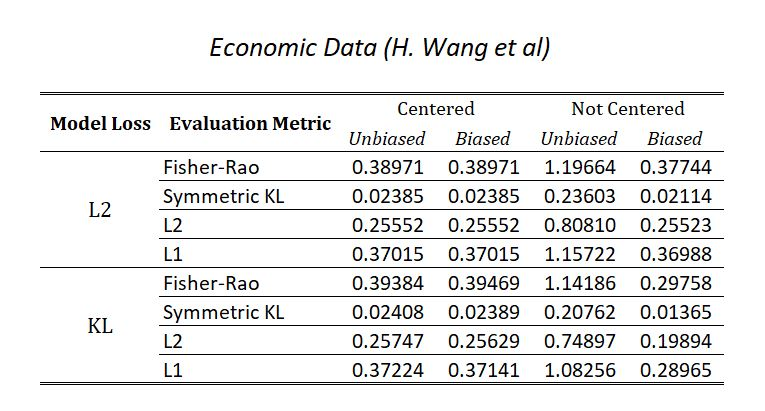
\includegraphics[scale=0.9,keepaspectratio=true]{table1.JPG}
 % table1.JPG: 0x0 px, -2147483648dpi, 0.00x0.00 cm, bb=
 \caption{Performance for Economic Data set}
\end{figure}
\begin{figure}[hbt!]
 \centering
 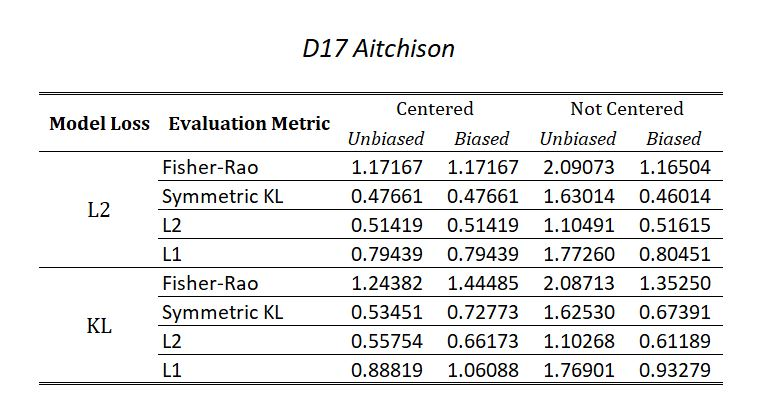
\includegraphics[scale=0.9,keepaspectratio=true]{table2.JPG}
 % table1.JPG: 0x0 px, -2147483648dpi, 0.00x0.00 cm, bb=
 \caption{Performance for D17}
\end{figure}
\newpage
\ \\
\
\begin{figure}[hbt!]
 \centering
 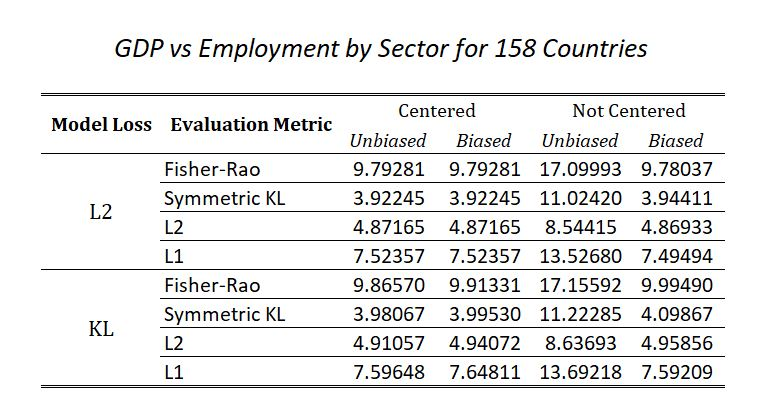
\includegraphics[scale=0.9,keepaspectratio=true]{table3.JPG}
 % table1.JPG: 0x0 px, -2147483648dpi, 0.00x0.00 cm, bb=
 \caption{Performance for GDP vs Employment Data set}
\end{figure}
\begin{figure}[hbt!]
 \centering
 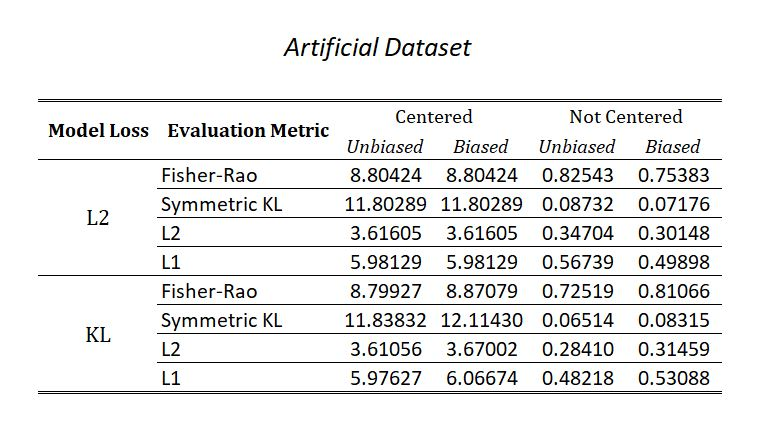
\includegraphics[scale=0.9,keepaspectratio=true]{table4.JPG}
 % table1.JPG: 0x0 px, -2147483648dpi, 0.00x0.00 cm, bb=
 \caption{Performance for Artificial Data set}
\end{figure}

\newpage

\begin{figure}
 \centering
 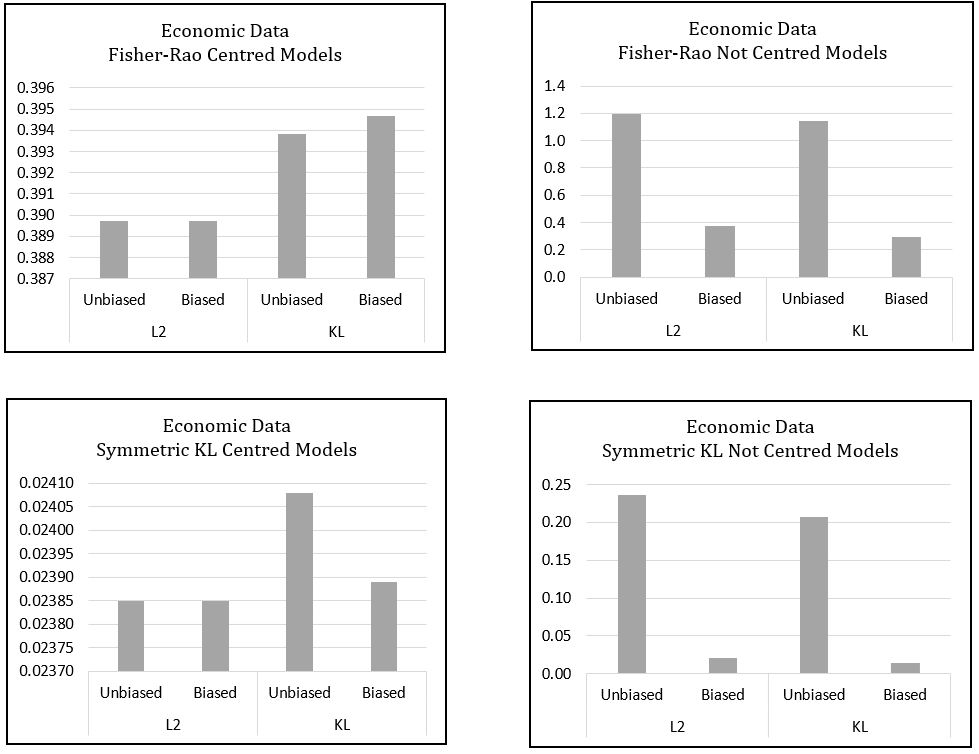
\includegraphics[scale=0.6,keepaspectratio=true]{graphs/G-Eco1.JPG}
 % G-Eco1.JPG: 0x0 px, 0dpi, 0.00x0.00 cm, bb=
 \caption{Performance against geometric measures (Economic data)}
\end{figure}

\begin{figure}
 \centering
 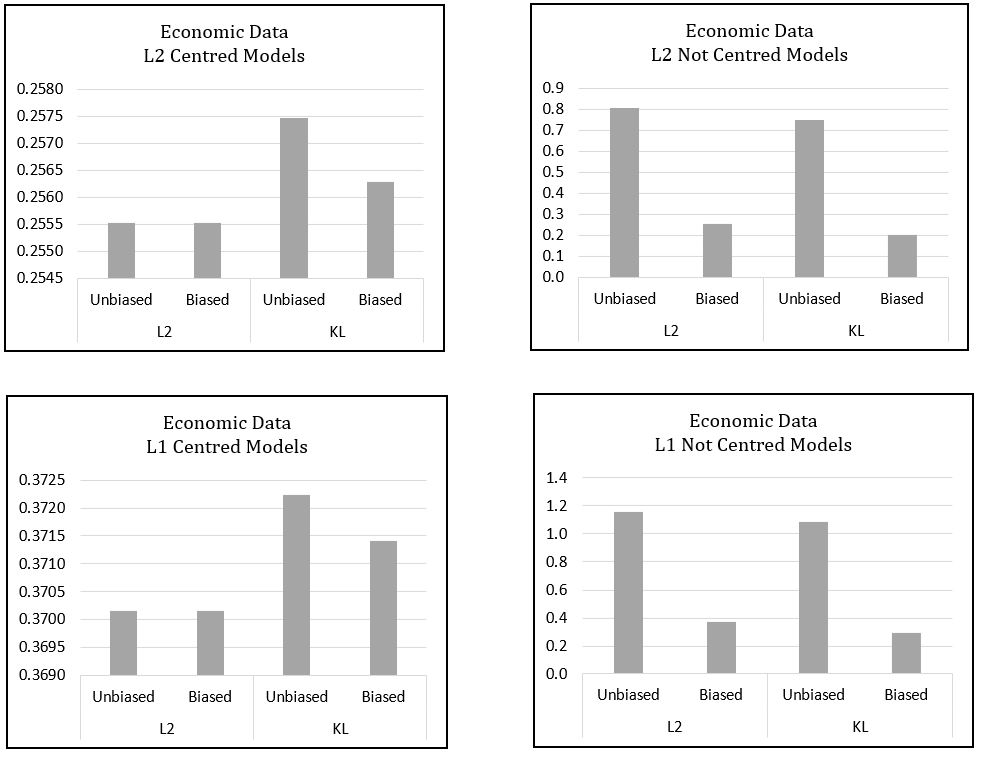
\includegraphics[scale=0.6,keepaspectratio=true]{graphs/G-Eco2.JPG}
 % G-Eco1.JPG: 0x0 px, 0dpi, 0.00x0.00 cm, bb=
 \caption{Performance against non-geometric measures (Economic data)}
\end{figure}

\newpage

\begin{figure}
 \centering
 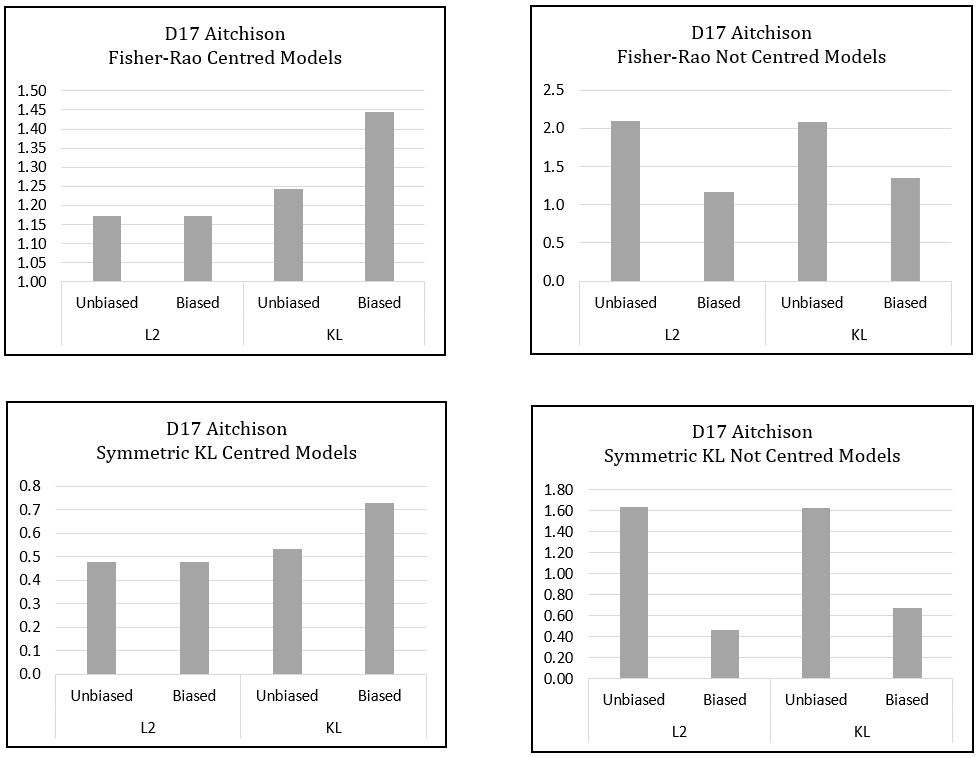
\includegraphics[scale=0.6,keepaspectratio=true]{graphs/G-D17-1.JPG}
 % G-Eco1.JPG: 0x0 px, 0dpi, 0.00x0.00 cm, bb=
 \caption{Performance against geometric measures (D17)}
\end{figure}

\begin{figure}
 \centering
 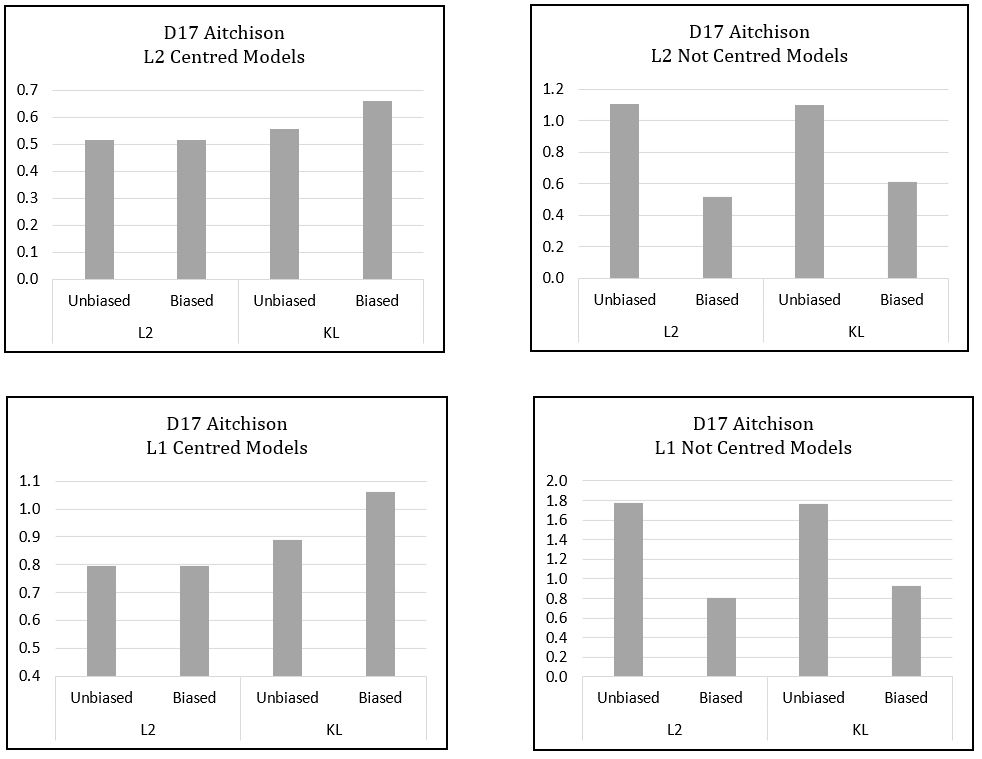
\includegraphics[scale=0.6,keepaspectratio=true]{graphs/G-D17-2.JPG}
 % G-Eco1.JPG: 0x0 px, 0dpi, 0.00x0.00 cm, bb=
 \caption{Performance against non-geometric measures (D17)}
\end{figure}

\newpage

\begin{figure}
 \centering
 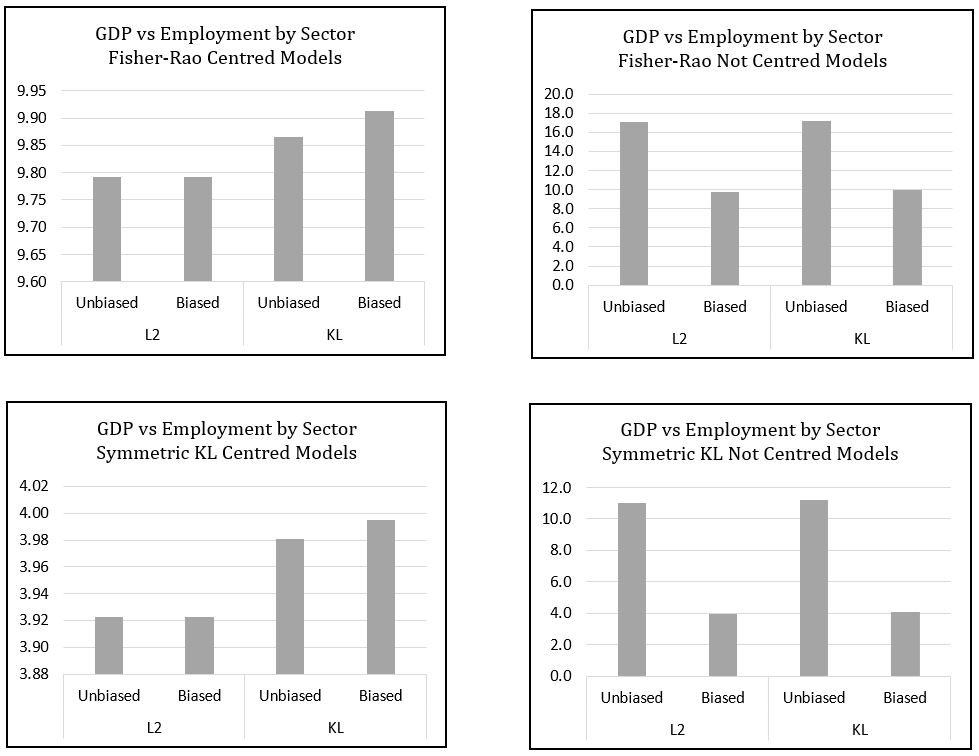
\includegraphics[scale=0.6,keepaspectratio=true]{graphs/G-GDP1.JPG}
 % G-Eco1.JPG: 0x0 px, 0dpi, 0.00x0.00 cm, bb=
 \caption{Performance against geometric measures (GDP vs Employment)}
\end{figure}

\begin{figure}
 \centering
 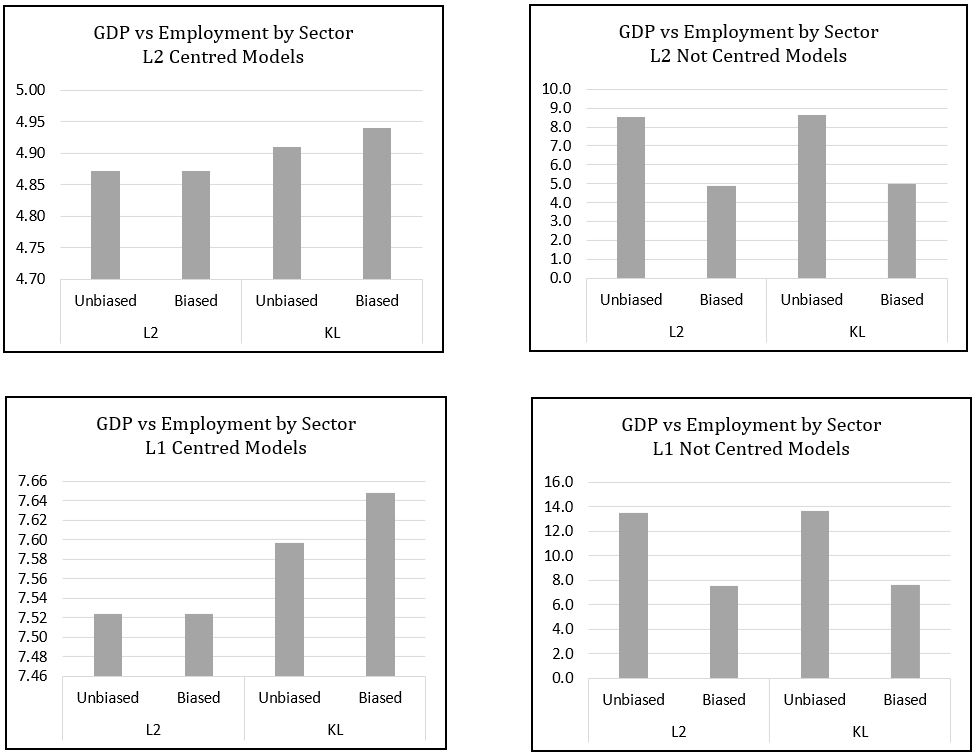
\includegraphics[scale=0.6,keepaspectratio=true]{graphs/G-GDP2.JPG}
 % G-Eco1.JPG: 0x0 px, 0dpi, 0.00x0.00 cm, bb=
 \caption{Performance against non-geometric measures (GDP vs Employment)}
\end{figure}
\newpage

\begin{figure}
 \centering
 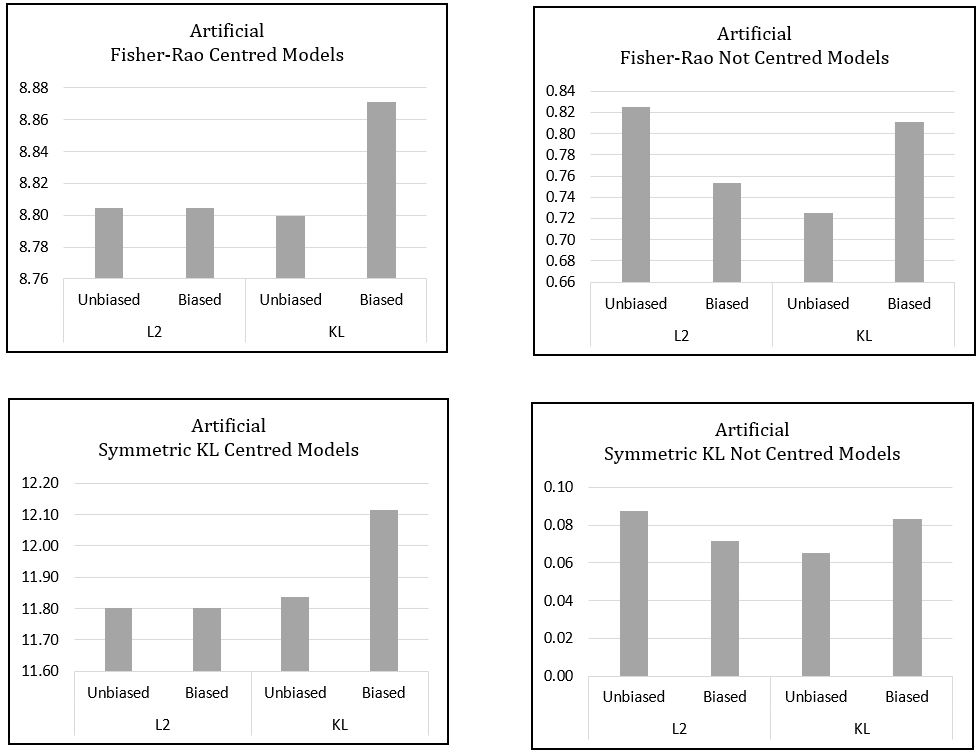
\includegraphics[scale=0.6,keepaspectratio=true]{graphs/G-Arti1.JPG}
 % G-Eco1.JPG: 0x0 px, 0dpi, 0.00x0.00 cm, bb=
 \caption{Performance against geometric measures (Artificial)}
\end{figure}

\begin{figure}
 \centering
 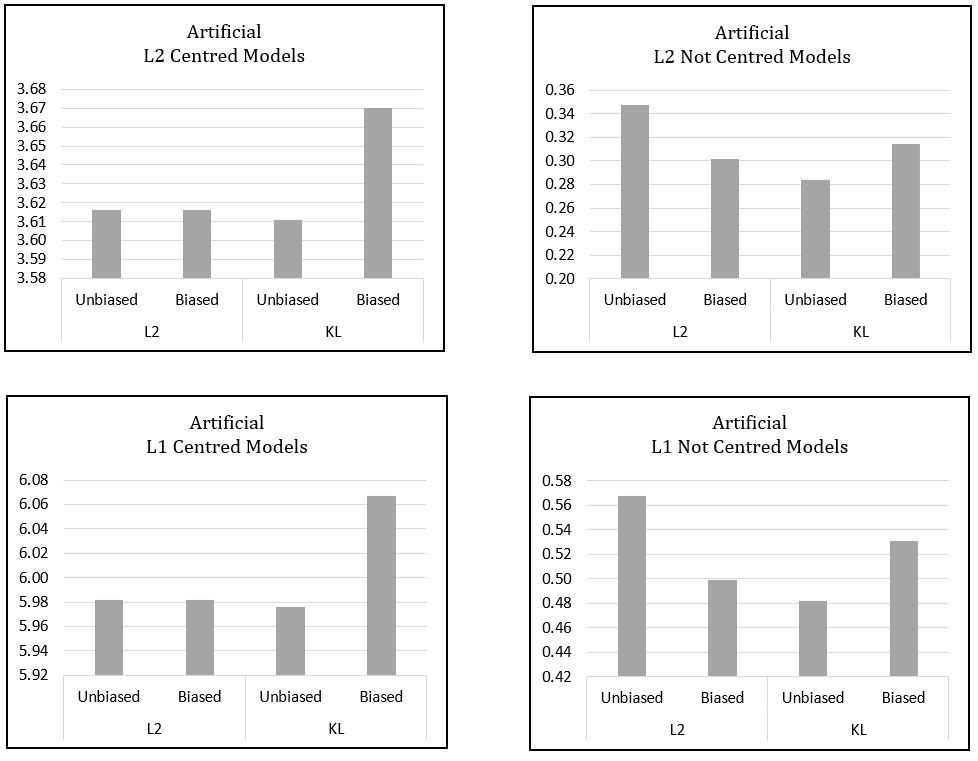
\includegraphics[scale=0.6,keepaspectratio=true]{graphs/G-Arti2.JPG}
 % G-Eco1.JPG: 0x0 px, 0dpi, 0.00x0.00 cm, bb=
 \caption{Performance against non-geometric measures (Artificial)}
\end{figure}

\newpage
\ \\
\section{Discussion}
\
First we note some broad observations.\\
\\

\begin{itemize}
 \item Although many of our models are generally competitive against Wang et al's (2013), they are usually slightly worse. The best models appear to be L2/unbiased/centred and L2/biased/non-centred. The only data set for which we can say some of our new models are significantly better is the artificial data set.\\
 \item We expected that the ranks of the models may shuffle as we move from geometric error measures to non-geometric ones, however the ranks tend to remain consistent.\\
 \item On the real data sets, not centralising consistently degrades the performance by a factor of 2. This is dramatically reversed on the artificial data set.\\
 \item On the real data sets, adding a bias term to non centralising models consistently improves performance by a factor of 2. \\
 \item If we centre the data, the biased and unbiased models with L2 loss give identical results.\\
 \item If we centre the data and use the KL loss, adding a bias term generally degrades the performance of the model (only the Economic data has counterexamples to this).\\ 
\end{itemize}

The fact that biased and unbiased L2 models give identical results when we centre the data is most likely not an accident. Printing the coefficients in the notebook shows that the biased model learns bias terms on the order of  $10^{-17}$ and non-bias terms very similar to the unbiased model. It could possibly be proven that the exact value of the bias term in this case is always zero. This would be interesting, as the corresponding theorem in the standard multivariate linear regression (that normalising the data so each variable has zero mean will produce an exactly zero bias term) is notably not true.\\
\\
The trends we observed that including a bias term somewhat balanced not centralising (and vice versa) were not surprising. We thought however that the L2/biased/not-centred model would slightly but noticeably outperform the L2/unbiased/centred model, but they tend to show very similar performance.\\
\\
We expected the KL loss models to perform well, at least in the geometric measures, but it was only slightly better in the Economic data set and slightly worse for the other 2 real data sets. Our reason for including the artificial data set was to show a case where the KL-loss models did indeed outperform the L2 loss models. Knowing that such data sets exist, it would be interesting to find a characterisation of such data sets, as understanding those characteristics would potentially allow us to predetermine whether the KL-loss will outperform L2-loss models for a particular problem. Investigating what makes our artificial data set so different to the real data sets would likely help us in finding such a characterisation.\\




\chapter{Conclusion}
In this project we have investigated the problem of performing regression with compositional data, with particular focus on Aitchison Simplex Regression. Motivated by arguments from information geometry, we considered a new gauged-KL loss for this problem, as well as including or excluding bias terms and centralisation of the data. In total we implemented efficient algorithms for 8 models, 7 of them being new models for Aitchison Simplex Regression. Experimenting with a range of data sets, we found our model with L2 loss, a bias term and no centralisation to be fairly competitive with the model introduced by Wang et al. (2013). We have also presented an artificial data set which demonstrates a situation where the KL loss models perform substantially better than L2 loss models and noted the vanishing of the bias term for L2 loss models on centred data on our data sets. \\
\\
Further work can be done towards giving proofs of the properties the bias term of these L2 loss models appears to satisfy. Additional, by further investigation of our artificial data set or otherwise, it may be possible to characterise for which types of data sets our KL loss models would outperform the L2 loss models. More study is also required of the Matrix Coefficient models discussed in Section 3.4. Such models would most likely be effective in the case of large $d$ data sets (such as those arising in genomics) as the currently investigated models (which can only have up to $d-1+m$ parameters) can not capture complicated relationships between many independent variables with many components. Sourcing high quality data sets with a large number of samples would be of great benefit in experimenting with the matrix coefficient models.

%% Bibliography %%
\begin{thebibliography}{0}

\bibitem{Aitchison82}
{\sc Aitchison, J 1982}, 'The statistical analysis of compositional data (with discussion)', Journal of the Royal Statistical Society B, Volume 44(2), pp. 139-177.

\bibitem{Aitchision86}
{\sc Aitchison, J 1986}, 'The Statistical Analysis of Compositional Data', Chapman and Hall, New York.

\bibitem{AitchisionEgozcue}
{\sc Aitchison, J \& Egozcue, J.J 2005}, 'Compositional data analysis: where are we and where should we be heading?', Mathematical Geology, Volume 37(7), pp. 829-850.

\bibitem{AitchisionShen}
{\sc Aitchison, J \& Shen, S.M 1980}, 'Logistic-normal distributions: some properties and uses', Biometrika, Volume 67(2), pp. 261-272.

\bibitem{Amari16}
{\sc Amari, S.I 2016}, 'Information Geometry and its Applications', Spinger-Verlag, Berlin.

\bibitem{Avalos16}
{\sc Avalos-Fernandez, M, Nock, R, Ong, C.S, Rouar, J, \& Sun, K 2016}, 'Representation Learning of Compositional data', NIPS'18 Proceedings of the 32nd International Conference on Neural Information Processing Systems. 

\bibitem{Boyd}
{\sc Boyd, S \& Vandenberghe, L 2004}, 'Convex Optimization', Cambridge University Press, Cambridge.

\bibitem{Dowty}
{\sc Dowty, J.G 2018}, 'Chentsov's theorem for exponential families', Information Geometry, Volume 1(1), pp. 117-135.

\bibitem{Egozcue03}
{\sc Egozcue, J.J, Pawlowsky-Glahn, V, Mateu-Figueras, G \& Barcelo-Vidal, C 2003}, 'Isometric logratio transformations for compositional data analysis', Mathematical Geology Journal, Volume 35, pp. 279-300.

\bibitem{Nock18}
{\sc Nock, R, Menon, A \& Ong, C.S 2018}, 'A scaled Bregman theorem with applications', NIPS'16 Proceedings of the 30th International Conference on Neural Information Processing Systems. 

\bibitem{Wang13}
{\sc Wang, H, Shangguan, L, Wu, J, \& Guan, R, 2013}, 'Multiple linear regression modelling for compositional data', J. Neurocomputing, Volume 122, pp. 490-500.

\bibitem{Wiki}
{\sc Wikipedia 2019}, 'List of countries by GDP sector composition', Wikipedia, viewed 31 May 2019, \text{<https://en.wikipedia.org/wiki/List\_of\_countries\_by\_GDP\_sector\_composition>}.



\end{thebibliography}

\chapter*{Appendix}
\section*{Project Description}
Compositional data is a type of data which conveys information about relative proportions rather than absolute measures. Applying classical machine learning methods to compositional data directly often performs very poorly or fails completely as it fails to take into account the special nature of the data. In this project we will investigate a regression problem involving compositional data and find applications of Bregman divergences to them. The results of this will be contained in the research report. We will also create a Jupyter notebook showcasing our techniques for machine learning on compositional data.\\

\subsection*{Learning Objective}
\ \\
\begin{itemize}
 \item Gain a solid understanding of the theoretical foundations behind a modern ML algorithm.\\
 \item Develop ability to find practical research questions extending the current literature and to do research.\\
 \item Gain competence in the Machine Learning coding workflow (data collection/cleaning, implementing algorithms, training, evaluation).\\
 \item Gain skills in writing an academic report.\\
 \item Gain experience in giving an academic presentation.\\
 
\end{itemize}



\subsection*{Assessed Components}
\ \\
\begin{itemize}
 \item Research Report : \ 75 \% of total mark \\
 \item Jupyter Notebook: 15 \% of total mark \\
 \item Presentation: \ \ \ \ \ \ \  \ \ 10\% of total mark \\
\end{itemize}

\newpage
\
\section*{Description of Project Artefacts}
To supplement this report we have submitted 4 files:\\
\begin{itemize}
 \item COMP8755\_Notebook.ipynb \\
 \item compositional\_data sets.py \\
 \item error\_metrics.py \\
 \item gdp\_wiki.csv \\
\end{itemize}

All of the code in these files were implemented by me. The data sets in these files were sourced from several sources (cited in the files) and entered and/or processed by me.\\

All experiments were run on a Intel Core i7 4930MX CPU and Ubuntu 16.04 operating system. The following software was used:\\

\begin{itemize}
 \item Anaconda Python Distribution 2019.03\\
 \item Python 3.6\\
 \item scipy 1.2.1\\
 \item numpy 1.16.2\\
 \item pandas 0.22.0\\
 \item scikit-bio 0.5.4\\
 
\end{itemize}


\newpage
\

\section*{README.txt}


\begin{verbatim}
This folder contains a Jupyter notebook which contains implementations
for the models discussed in the report and produces evaluations of
those models on 4 compositional data sets. 

The notebook relies on 3 other files:
error_metrics.py contains the metrics with which we evaluate our models
compositional_data sets.py and gdp_wiki.csv allow us to retrieve our
data sets from within the notebook in a convenient manner.

To be able to run the code:
1) Install the Anaconda Python Distribution

2) Create a new environment with the following terminal commands:
>>> conda create -n coda_env python=3.6 scipy numpy pandas scikit-bio

If any issues running the notebook, specify the following versions:
python=3.6 scipy=1.2.1 numpy=1.16.2 pandas=0.22.0 scikit-bio=0.5.4

3) Activate that environment with the command:
>>> activate coda_env

4) Root a terminal session inside the folder and launch Jupyter:
>>> jupyter notebook

5) Open COMP8755_Notebook.ipynb and run all cells. 


All code submitted is completely my own work. 

\end{verbatim}


\end{document}

